\chapter{Monte Carlo Methods}
\label{chap:qmc}

% probably get some inspiration from Kai's and Werner's theses -- focus on FCIQMC

\gls{MC} methods are a class of numerical methods that use random sampling to numerically solve problems. It has found applications in an impressive range of fields, from physics to finance.\supercite{boyleOptions1977,johnsonMonte2024,kroeseWhy2014,rosenbluthMonte1955,foulkesQuantum,thijssenComputational2007}
It is particularly useful for problems with high dimensionality, where deterministic methods are often impractical. In quantum chemistry and physics, since a `dimension' can refer to any degree of freedom, high-dimensional problems are commonplace, and so \gls{MC} methods are a natural choice.

While the name \emph{Monte Carlo} was coined by Stanislav Ulam, after the famous casino in Monaco,\supercite{metropolisMonte1949,metropolisEquation1953} the foundational concept was already developed in the 18th century by the French mathematician Georges-Louis Leclerc, Comte de Buffon. As one of the earliest example applications, in the Buffon needle problem, one can randomly toss needles onto a lined sheet of paper and determine $\pi$.\supercite{leclercEssai,Histoire1735,senetaNineteenthCentury2001}

Monte Carlo methods is a broad term, and as such it is not possible to give a comprehensive overview in a single chapter, and there exist many reviews and textbooks on \gls{MC} and related topics.\supercite{allenComputer1989,binderMonte1986,binderMonte1988,newmanMonte1999,reiherHammersley1966,barKalos1988}
Here, we will focus on only a few concepts particularly relevant for this dissertation, largely following reference \citenum{foulkesQuantum} and the relevant chapters of reference \citenum{thijssenComputational2007}.

\section{Classical Monte Carlo Methods}

We start our discussion with classical \gls{MC} methods. While there are numerous possible applications, notably in molecular dynamics,\supercite{allenComputer1989} here we restrict ourselves to the topic of Monte Carlo integration. In particular, we consider the classical textbook problem of calculating the value of $\pi$, then we provide a more rigorous framework.

\subsection{A Very Bad Game of Darts}

If we imagine throwing darts at a dartboard randomly, we can approximate $\pi$. If the radius of the circle is $r$, then its area is $\pi r^2$. The area of the square circumscribing the circle is $4r^2$. Therefore, the ratio of the area of the circle to the area of the square is $\pi/4$. If we randomly sample a point in the square (``throw a dart''), the probability that the point is inside the circle is proportional to its area. Since we sample inside the square, the probability of landing inside the circle is
\begin{equation}
    P(\text{inside circle}) =  \frac{\pi r^2}{4r^2} = \frac{\pi}{4}.
\end{equation}
Therefore, if we sample a large number of points, the ratio of the number of darts that land inside the unit circle to the total number of darts, we can approximate the probability distribution $P$ and thus get an estimate for $\pi$ as
\begin{equation}
    \pi\approx 4\frac{N_\mathrm{in}}{N_\mathrm{out}}.
\end{equation}
This is illustrated in figure \ref{fig:darts}, and captures the core philosophy of \gls{MC} methods.

\begin{figure}[htbp]
    \centering
    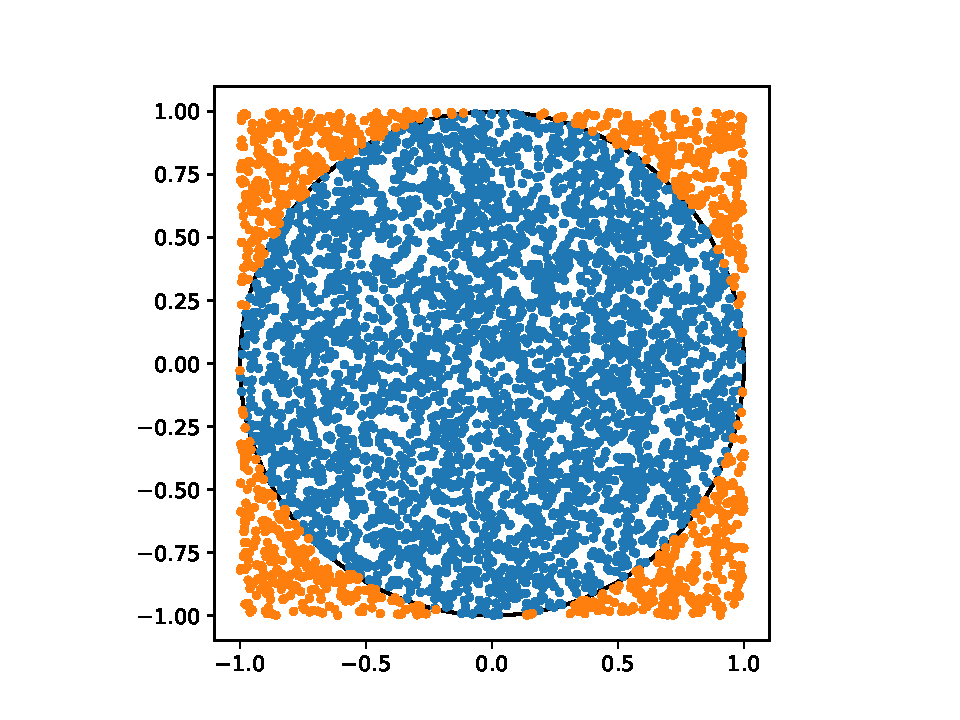
\includegraphics[width=\textwidth]{figures/qmc/darts.pdf}
    \caption{Our ``game of darts''. Points inside the unit circle are coloured blue whereas points outside are orange. Using stochastic sampling, this naive approach uses 5000 randomly generated coordinates $(x,y)\in[-1,1]\times[-1,1]$ to approximate $\pi\approx 4N_\mathrm{in}/N_\mathrm{out}\approx 3.1464$.
    % Of course, there are many ways to improve this method, the most obvious being to use a fraction of the unit circle, such as the first quadrant.
    }
    \label{fig:darts}
\end{figure}

Controlling the stochastic error is critical in \gls{MC} methods. To estimate the reliability of our estimate, we can determine the standard deviation of the estimate. Our sampling scheme is a binomial distribution, with $p=\pi/4$. Hence,
\begin{equation}
    \sigma^2_{\pi} = \mathrm{Var}(4P(\text{inside circle})) = \frac{16p(1-p)}{N}
\end{equation}
or
\begin{equation}
    \sigma_\pi
    = 4\sqrt{\frac{\frac \pi 4 (1-\frac \pi 4)}N}
    \propto \frac{1}{\sqrt{N}}.
\end{equation}

\subsection{A More Mathematical Description}

As we have expressed the problem of the previous section in terms of areas, it is clear that it can also be formulated in terms of integrals. For this particular problem, we have:
\begin{equation}
    \pi = \int_{-1}^1  \mathrm{d}x \int_{-1}^1 \mathrm{d}y\ \Theta(1-x^2-y^2) ,
\end{equation}
where $\Theta$ is the Heaviside step function.
More generally, consider the integral of some smooth function $f$ over $[a,b]\subseteq \mathbb{R}$,\footnote{We present the one-dimensional case for simplicity. The generalization to higher dimensions is straightforward.}
\begin{equation}
    I = \int_a^b \d x \ f(x).
\end{equation}
Standard finite element methods for solving integrals of this type typically involving dividing the integration domain into $N$ subintervals of length $h$ and determining the weights $w_i$ from e.g. a polynomial approximation. That is,
\begin{equation}
I \approx \sum_{i=1}^N w_if(x_i).
\end{equation}
The error $\sigma$ in these sorts of methods is typically $\sigma\propto h^{-k} \propto N^{-k}$, where $k\in\mathbb{Z}_{>0}$. For a multi-dimensional integral, $\sigma\propto N^{-k/d}$, where $d$ is the number of dimensions.\cite{ascherFirst2011}
% I am mostly following the discussion and notation in Thijssen's book -- remember to cite it along with all the primary references

In \gls{MC} methods, $\forall i$ take $w_i=1$ and $x_i\in[a,b]$ randomly sampled. That is,

\begin{equation}
    I\approx \sum_{i=1}^N f(x_i).
\end{equation}
If, for example, we choose $N$ to be randomly sampled, then the variance is
\begin{align}
    \sigma^2 &= \left\langle \left( \frac{b-a}{N}\sum^N_{i=1}f_i\right)^2\right\rangle - \left( \left\langle  \frac{b-a}{N}\sum^N_{i=1}f_i\right\rangle\right)^2 \\
    &= \frac{(b-a)^2}{N}(\bar{f^2} - \bar f^2)
\end{align}
where $f_i\mathdef f(x_i)$ and $x_i$ is a random number drawn, the angular brackets denote an average over all possible realisations, and the overbar represents an average of the function over the domain ($[a,b]$ in this discussion). i.e. the error in this method is proportional to the variance of $f$. Perhaps more interestingly, $\sigma\propto N^{-1/2}$, in line with the central limit theorem.\supercite{bernoulliJacobi1713} Comparing this error with standard quadrature, we see that MC integration is more efficient than an order-$k$ algorithm when $d>2k$. That is, although this particular \gls{MC} example is naive, using simply a uniform distribution, it is still more efficient than standard methodologies for very large dimensions.

There exist several methods to reduce errors in \gls{MC} methods.\supercite{jamesMonte1980} Among the most important ones is importance sampling.\supercite{kahnModification1959} In the prevous example, it is clear that if significant contributions to the integral come from a small region of the domain, only a few points would be sampled by the \gls{MC} algorithm there when using a uniform distribution. This would lead to large statistical errors. Mathematically, this is from the large variance of the function. In importance sampling, we sample from a distribution $p$ which has roughly the same shape as $f$ such that $f/p$ is roughly constant over the integration domain. Of course, being a probability distribution, we require
\begin{equation}
    p(x)>0 \quad \forall x
\end{equation}
and
\begin{equation}
    \int\d x \ p(x) = 1.
\end{equation}

The integral is
\begin{equation}
    I = \int\d x \  f(x) = \int\d x\ \frac{f(x)}{p(x)} p(x).
\end{equation}
Then, if we sample points according to $p$, we have
\begin{equation}
    I\approx \frac{1}{N}\sum^N_{i=1} \frac{f(x_i)}{p(x_i)},
\end{equation}
where the naive \gls{MC} method is recovered when $p(x)=1/(b-a)$, i.e. the uniform distribution.

In this case, the variance in the result is
\begin{equation}
    \sigma^2 = \left\langle \left( \frac{1}{N}\sum^N_{i=1} \frac{f(x_i)}{p(x_i)}\right)^2\right\rangle - \left( \left\langle  \frac{1}{N}\sum^N_{i=1} \frac{f(x_i)}{p(x_i)}\right\rangle\right)^2.
\end{equation}
From this, we can see that if $f/p$ is constant, the error vanishes, so it is important to choose a good $p$. If $p$ is chosen poorly, the variance can be worsened, so this is a delicate problem.

In practice it is often difficult to estimate $f$, and a choice for $p$ is problem-specific. However, when we have some approximation for its overall shape, importance sampling can be a powerful tool. Alternatively, another method known as adaptive Monte Carlo\cite{arounaAdaptative2004} seeks the most significant regions of $f$ by random sampling, so that no a priori knowledge of the functional form is required.

\subsection{Metropolis-Hastings Algorithm}
\label{sec:mcmc}
A particularly successful method for generating random samples $x_i$ from a probability distribution $\pi(x)$, where direct sampling of $\pi$ is difficult, is the Metropolis-Hastings algorithm.\supercite{metropolisEquation1953,hastingsMonte1970} Often, $\pi(x)$ is known only up to a normalisation constant, $\pi(x)=\pi(x)/C$ where $C=\int\d x\ \pi(x)$ is intractible.

The Metropolis-Hastings algorithm is based on Markov chains,\supercite{markovTheory1954} and we construct such a Markov chain so that its stationary distribution is $\pi(x)$, which is to say if the Markov chain starts at $\pi(x)$ for step $t$, it is still $\pi(x)$ for step $t+1$.

The probability of having a sequence of states $x_1,x_2,\ldots,x_N$ is
\begin{equation}
    p(x_1,x_2,\ldots,x_N) = p(x_1)p(x_2|x_1)p(x_3|x_2)\cdots p(x_N|x_{N-1}).
\end{equation}
where $p(x|x')$ is the transition probability from $x'\to x$. Then, the probability at step $t$ to be in state $x$, $\pi_t(x)$ is given by
\begin{equation}
\pi_{t+1}(x) = \sum_{x'\in \Omega} \pi_t(x')p(x|x')
\end{equation}
where $\Omega$ is the set of all possible states. This is called the master equation. In the stationary state, $\pi_t(x)=\pi(x)$, so
\begin{equation}
    \pi(x) = \sum_{x'\in \Omega} \pi(x')p(x|x').
\end{equation}
Finding the general solution to this problem is nontrivial. However, a sufficient (but not necessary) condition is called detailed balance:
\begin{equation}
    \pi(x)p(x|x') = \pi(x')p(x'|x).
\end{equation}
This ensures that the probability of going from $x$ to $x'$ is the same as the probability of going from $x'$ to $x$, which implies that the probability is stationary.

In order to actually construct the algorithm, we must introduce the trial step probability $\omega(x|x')$, and the acceptance probability $A(x|x')$. Then,
\begin{equation}
    p(x|x') = \omega(x|x')A(x|x').
\end{equation}
$\omega(x|x'),A(x|x')\in [0,1]$ for each pair $x,x'$, and $\sum_{x'}\omega(x|x') = 1$. Furthermore, the original formulation of the algorithm required $\omega(x|x') = \omega(x'|x)$, which leads to (plugging into the master equation)
\begin{equation}
    \frac{A(x|x')}{A(x'|x)} = \frac{\pi(x')}{\pi(x)}.
\end{equation}

The algorithm proceeds in two stages: we propose a step $x'\to x$, and then accept or reject it. The probability of accepting is
\begin{equation}
    A(x|x') = \min\left(1,\frac{\pi(x')}{\pi(x)}\right).
\end{equation}
If we accept, we set the new state to $x$, otherwise we stay at $x'$.

In practice, on a computer, accepting is done by generating a uniform random number $r\in [0,1)$ and accepting if $r<\frac{\pi(x')}{\pi(x)}$, and otherwise rejecting. Furthermore, we don't just have a single Markov chain, but a collection of so-called ``walkers'', that each perform their own Markov chain (for parallelisation). The integrand is then sampled at each position where the walkers reach.

One final note, is that since the current state of a Markov chain is dependent on the previous state, the Markov chain is not independent of itself. This is referred to as autocorrelation. One method to reduce this autocorrelation and give essentially independent samples is known as blocking.\supercite{flyvbjergError1989}

\section{Variational (Quantum) Monte Carlo}
\label{sec:vmc}

As our first foray into \gls{QMC}, we consider \gls{VMC}. In section \ref{sec:variational_principle} we introduced the Variational Principle by parametrising the wave function and then finding the minimum of the expectation value of the energy occurring in the parametrisation space. If we have a large number of electrons and/or a large number of parameters, then the integrals involved in the evaluation of the energy will necessarily be high-dimensional. This is where \gls{MC} comes in. For basic trial wave functions and small atoms like Hydrogen or Helium, direct integration may be possible, but as discussed in the previous section, this quickly becomes impossible for larger systems.

For a trial wave function $\Psi$ (we omit the tilde from section \ref{sec:variational_principle}), the expectation value of the energy is
\begin{align}
    \label{eq:vmc_energy}
    \langle E \rangle &= \frac{\bra{\Psi}H\ket{\Psi}}{\bra{\Psi}\ket{\Psi}} \\
    \label{eq:vmc_step1}
    &= \frac{\int\d^{3N}r\ \Psi^*H\Psi}{\int\d^{3N}r\ |\Psi|^2} \\
    \label{eq:vmc_step2}
    &= \frac{\int\d^{3N}r\ \Psi^*\Psi \frac{H\Psi}{\Psi}}{\int\d^{3N}r\ |\Psi|^2} \\
    \label{eq:vmc_step3}
    &= \frac{\int\d^{3N}r\ |\Psi|^2 E_L(\bm r)}{\int\d^{3N}r\ |\Psi|^2},
\end{align}
where we have introduced the local energy, defined as
\begin{equation}
    E_L(\bm r) \mathdef \frac{H\Psi}{\Psi}.
\end{equation}
This rewriting of the integral is particularly suitable for evaluation using \gls{MC}. Then we may vary the parameters and stop according to some minimisation algorithm.
Notice that the more strongly $\Psi$ resembles the exact wave function, the less strongly $E_L$ varies with $\bm r$. In particular, if $\Psi$ is equal to an exact eigenstate, then $E_L$ is constant. Therefore, an alternative objective function to the energy expectation of equation \ref{eq:vmc_energy} is the variance.\supercite{cuzzocreaVariational2020,snajdrAre2000,kentMonte1999}

Defining
\begin{equation}
    p(\bm r) = \frac{|\Psi|^2}{\int\d^{3N}r\ |\Psi|^2},
\end{equation}
we may write equation \ref{eq:vmc_energy} as
\begin{equation}
    \langle E\rangle = \int\d^{3N}r\ p(\bm r)E_L(\bm r).
\end{equation}

This form of the energy is amenable to the Metropolis-Hastings approach outlined in section \ref{sec:mcmc}. Recall also that $p$ need not be normalised when using the Metropolis-Hastings algorithm for sampling.

In principle, the algorithm is doable with just a single walker, but in practice we reduce the statistical error by using many. The algorithm then becomes

% \begin{minipage}{\textwidth}
\begin{lstlisting}[escapeinside={(*}{*)}]
    Initialise (*$N$*) walkers in random positions.
    until convergence criterion met(*\footnote{The convergence criterion in VMC is typically just to sample a predefind number of configurations.}*)
      for each walker at position (*$r$*)
        sample the local energy (*$E_L$*) at (*$r$*)
        propose a new position (*$r'$*) with probably (*$p=|\Psi(r')/\Psi(r)|^2$ *)
        if (*$r'$*) is accepted
          set (*$r$*) to (*$r'$*)
\end{lstlisting}
% \end{minipage}

The energy is then calculated as the expectation value of the local energy, averaged over the samples generated in this procedure. Steps at the beginning (before equilibrium) are discarded in a process called equilibration,\supercite{casino} and a blocking procedure should be employed. The decision to stop is generally based on compute time and/or precision required.

\subsection{Trial Wave Functions}
\label{sec:jastrow}

While \gls{VMC} is a powerful tool, the quality of the solution is constrained by the quality of the trial wave function. Moreover, the evaluation of the trial wave function is expensive, and we therefore want a form that is easy to evaluate.

The form of the trial wave function is typically chosen based on a Jastrow factor, as already introduced in section \ref{sec:tc}. Generally,\supercite{jastrowManyBody1955}
\begin{equation}
    \label{eq:slater-jastrow}
    \Psi_\mathrm{trial} = \e^J\Phi.
\end{equation}

For computational efficiency, the Jastrow factor typically only retains one- and two-body terms,\supercite{foulkesQuantum}
\begin{equation}
    J = \sum_i \chi(\bm x_i) - \frac 12 \sum_{i\neq j} u(\bm x_i, \bm x_j),
\end{equation}
where $\chi$ describes electron-nuclear correlation and $u$ describes two-electron correlation (including e.g. electron-electron-nuclear correlation). There exist a number of more specific forms for $J$,\supercite{lopezriosFrameworkConstructingGeneric2012} though one unifying principle is for them to adhere to expected short-range (cusp conditions) and long-range ($1/r$) behaviour.

$\Phi$ is typically chosen to be a single Slater determinant.\supercite{foulkesQuantum,fahyVariational1988,liCohesive1991,rajagopalQuantum1994,malatestaVariational1997}
In particular, by choosing the \gls{HF} determinant, typically only a small portion of the energy (that is, the correlation energy) is left for the Jastrow factor to describe, and typically even simple Jastrow factors can do this.\supercite{foulkesQuantum}
However, sometimes this is not enough, for example, when the HF determinant is not sufficient to describe all symmetries of the true wave function.\supercite{harrisonQuantum1985,lesterRecent1997,umrigarDiffusion1993}

\section{Diffusion Monte Carlo}
\Gls{DMC} starts by performing a Wick rotation (that is, substitute $t\to i\tau$) on the time-dependent Schr\"odinger equation, equation \ref{eq:schrodinger}. We then get the imaginary-time Schr\"odinger equation
\begin{equation}
    \label{eq:imag_time_schrodinger}
    \frac{\partial}{\partial\tau}\Psi(\bm r, \tau) = -\hat H \Psi(\bm r, \tau).
\end{equation}
This equation is a diffusion (or heat) equation, and $\Psi$ may be interpreted as the density distribution for a large number of independent particles\footnote{Note that the particles, henceforth referred to as walkers, are not the particles being described by the Hamiltonian. One walker represents a configuration of all the particles described by the Hamiltonian.} (walkers).\supercite{fickLiquid1995}
More specifically, the kinetic energy term, being second order, describes the movement of the walkers whereas the potential energy term describes generation or annihilation of walkers. The solution of this equation is
\begin{equation}
    \Psi(\bm r, \tau) = \e^{-(\hat H-S)\tau}\Psi(\bm r, 0),
\end{equation}
where we have introduced the energy shift $S$ which is adapted throughout the simulation every $n$ steps to keep the number of walkers constant, and to estimate the ground state energy.\supercite{kosztinIntroduction1996} In particular, if we expand $\Psi(\bm r, 0)$ in terms of the eigenfunctions of $\hat H$, $\{\psi_i\}$, labeled in such a way that $i>j\implies E_i>E_j$, we get
\begin{equation}
    \label{eq:imag-time-decay}
    \Psi(\bm r, \tau) = \sum_{i}a_i\e^{-(\hat E_i-S)\tau}\psi(\bm r).
\end{equation}
Here, $a_i$ is the coefficient of the $i$th eigenfunction, and $\hat E_i$ is the corresponding eigenvalue. After the excited-state solutions have decayed, the only possible value of $S$ that stabilises the simulation is $S=E_0$. It is also clear from equation \ref{eq:imag-time-decay} that when $S=E_0$, all excited states decay exponentially to zero, and we are left with the ground state for large $\tau$.

We may also express $\Psi$ in terms of its Green's function, in order to get a form that expresses a small time step,
\begin{equation}
\Psi(\bm r, \tau+\Delta\tau) = \int\d^{3N}r' \ G(\bm r, \bm r'; \Delta\tau)\Psi(\bm r, \tau),
\end{equation}
where the Green's function
\begin{equation}
G(\bm r, \bm r'; \Delta\tau) = \bra{r}\e^{-\Delta\tau(H-S)}\ket{r'}
\end{equation}
also obeys the imaginary-time Schr\"odinger equation, but with the initial condition
\begin{equation}
    G(\bm r, \bm r'; 0) = \delta(\bm r-\bm r').
\end{equation}

For small time steps, $G$ may be approximated by the Lie-Trotter-Suzuki decomposition,\supercite{lieTheorie1970,trotterProduct1959,suzukiGeneralized1976} i.e. for operators $A$, $A_k$,
\begin{equation}
    A = \sum_kA_k \implies \e^{-\alpha A} \approx \left( \prod_k e^{-\alpha A_k/M} \right)^M
\end{equation}
for some value $\alpha$ and for large $M$. From this, we can get the Green's function,
\begin{equation}
    G(\bm r, \bm r'; \Delta\tau) = \e^{-\Delta\tau(V(r)-S)}\frac{1}{\sqrt{2\pi\Delta\tau}}\e^{-(r - r')^2/(2\pi\Delta\tau)}+\mathcal{O}(\Delta\tau^2),
\end{equation}
which describes our time evolution.

In \gls{DMC}, walkers diffuse through configuration space in two stages: diffusion and branching. In the diffusion step, walkers are moved according to the kinetic terms in the Green's function. In the branching step, unfavourable walkers are removed and favourable ones produce new walkers.

For the energy shift estimate, we wish to choose a value such that the overall population does not change too much. If the walkers proliferate too much, then the computational cost becomes infeasible, whereas if too many walkers die, we are left with poor statistics. One way to choose $S$ is by keeping track of the population of walkers $N_w$ for a target populaton $N_w^\mathrm{target}$ and adjust,
\begin{equation}
    S = S_\mathrm{old} + \alpha\ln\left(\frac{N_w^\mathrm{target}}{N_w}\right)
\end{equation}
for small $\alpha$.

More concretely, in pseudocode, the basic \gls{DMC} algorithm is:

\begin{minipage}{\textwidth}
\begin{lstlisting}[escapeinside={(*}{*)}]
    Initialise (*$N$*) walkers in random positions.
    until convergence criterion met
        for each walker at position (*$\bm r$*)
            shift position (*$\bm r$*) to (*$\bm r'$*) according to
              (*$\hookrightarrow$*)transition probability (*$G$*)
            evaluate (*$q=\e^{-\Delta\tau(V(\bm r')-S)}$*)
            walker survives with probability (*$q$*)
            if (*$q>1$*)
                create (*$1-q$*) new walkers
                  (*$\hookrightarrow$*)(with stochastic rounding)
        update (*$S$*).
\end{lstlisting}
\end{minipage}

Notice that in contrast to \gls{VMC}, \gls{DMC} does not rely on a trial wave function. There is also a discretisation error incurred by the operator decomposition, though this can be handled via an application of the Metropolis-Hastings alogirthm.\cite{thijssenComputational2007}
However, in practice a trial wave function is actually necessary for fermions in order to improve the statistics. The walker distribution is positive, but for fermions this is not the case due to their exchange statistics. Since in electronic structure, we focus on fermions (electrons), this is an important feature. In order to still practically use DMC,\footnote{Other simple solutions such as assigning a sign to each walker leads to large errors.} an approximation called the fixed node approximation is made, where the nodal structure (i.e. the roots of $\Psi$) of the distribution is determined by a trial function. Thus, the accuracy of DMC is still limited by the quality of the trial wave function (or more precisely, by its nodal surface). In a Slater-Jastrow-type trial wave function like equation \ref{eq:slater-jastrow}, only the Slater-component will affect the nodal surface (and hence the accuracy). Thus, the choice of orbitals as well as the number of determinants can be important considerations.

% While \gls{DMC} does not rely on the variational principle, the convergence of its practical variants still relies on a trial wave function.


% \section{Auxiliary Field Quantum Monte Carlo}
% % may can skip AFQMC? Don't really see a point to including a full discussion of this method
% \section{The Fermion Sign Problem}
% \label{sec:sign_problem}
% maybe can also skip the fermion sign problem since it's not super relevant for me, just mention it vaguely in the DMC section

\section{Full Configuration Interaction Quantum Monte Carlo}
\label{sec:fciqmc}

The main post-Hartree-Fock method used throughout this dissertation is the \gls{FCIQMC} algorithm.\supercite{booth_fciqmc_2009} For this, there exist a few different implementations,\cite{Guther_neci_2020,spencerHANDEQMC2019b,brandRimujl2024,andersonRobertanderson2024} but we focus on \neci.\cite{Guther_neci_2020} As the name implies, \gls{FCIQMC} combines concepts from \gls{FCI} (discussed in section \ref{sec:ci}) and \gls{QMC} concepts already discussed in this chapter. In particular, it implements FCI, retaining many of its desirable properties such as size consistency and accuracy while being able to handle much larger systems thanks to its stochastic framework (however, the scaling remains exponential, like FCI). Like FCI, it is non-perturbative, and so can handle multi-reference problems, and unlike other QMC methods, it does not rely on a trial wave function. It can also be used as a solver in place of FCI, like in a \gls{MCSCF} calculation.\supercite{dobrautzSpinPure2021,weserStochastic2022}

\subsection{Main Concepts}

Like \gls{DMC}, \gls{FCIQMC} is based on the imaginary-time Schr\"odinger equation, equation \ref{eq:imag_time_schrodinger}, repeated here:
\begin{equation}
    \frac{\partial}{\partial\tau}\Psi(\bm r, \tau) = -\hat H\Psi(\bm r, \tau).
\end{equation}
The solution to this equation is
\begin{equation}
    \Psi(\bm r, \tau) = \e^{-\tau\hat H}\Psi(\bm r, 0).
\end{equation}
Expanding $\e^{-\tau\hat H}$ to first order in small imaginary time step $\Delta\tau$ gives us the FCIQMC projector
\begin{equation}
    \label{eq:fciqmc_projector}
    P = 1-\Delta\tau\hat H \to 1-\Delta\tau(\hat H - S),
\end{equation}
where we have introduced an arbitrary shift $S$ in analogy to \gls{DMC}. Notice, in particular, that if $S=E_0$ the ground state energy, all other states decay away. Hence, repeated application of $P$ while adjusting $S$ to get as close to $E_0$ as possible will give us the ground state, as long as our initial state has nonzero overlap with the ground state.

Like \gls{FCI}, the wave function is expanded in some basis. Throughout this dissertation, \glspl{SD} are used, though \glspl{CSF} are also possible.\supercite{dobrautzEfficient2019} The basis will be kept constant, and the coefficients may change with each time step,
\begin{equation}
    \ket{\Psi(\tau)} = \sum_i c_i(\tau)\ket{D_i}.
\end{equation}

Like in \gls{DMC}, we adjust $S$ to approximate the ground state energy $E_0$, as $S=E_0$ would project out all states other than the ground state, as long as $\braket{\Psi(\tau=0)}{\Psi_0}\neq 0$ where $\ket{\Psi_0}$ is the ground state. Similarly, $S$ affects the walker population. In particular, for walker population $N_w$, if $S>E_0$ then the population grows, and if $S<E_0$ it decays. If we have a target population $N_w^\mathrm{target}$ then we keep $S>E_0$ (typically, just by setting $S=0$) and ``turn on'' the shift once $N_w^\mathrm{target}$ is reached. However, unlike DMC, \gls{FCIQMC} walkers can have either negative or positive weight. These weights correspond to the $c_i$, and the walkers ``diffuse'' across \gls{SD} (or \gls{CSF}) space. The walker population is reported in terms of absolute values, i.e.
\begin{equation}
    N_w = \sum_{i\in\{SDs\}}|N_i|,
\end{equation}
where we sum over the walkers across all \glspl{SD}. Once in variable-shift mode, in practice $S$ is updated every $m$ cycles:
\begin{equation}
    S(\tau+m\Delta\tau) = S(\tau) - \frac{\zeta}{m\Delta\tau}\ln\left(\frac{N_w(\tau+m\Delta\tau)}{N_w(\tau)}\right),
\end{equation}
where $\zeta$ is a damping parameter.

The key advantage of \gls{FCIQMC} over ordinary \gls{FCI} is no longer needing to store the full \gls{CI} vector, making use of sparsity. Even for relatively large and strongly-correlated systems, only a small subspace of the entire Hilbert space needs to be sampled in FCIQMC, whereas in FCI, the full CI vector must be stored (or if done via dense diagonalisation, the entire $H$ matrix, which is unrealistic for even small systems).

\subsection{Basic Algorithm}

\gls{FCIQMC} is typically run in three steps:
\begin{enumerate*}[label=(\alph*), itemjoin={\hspace{1em}}]
    \item \textbf{spawning},
    \item \textbf{death/cloning}, and
    \item \textbf{annihlation}.
\end{enumerate*}
Each step can be recognised in the application of the projector operator of equation \ref{eq:fciqmc_projector} onto some state
$\ket\Psi = \sum_i c_i\ket{D_i}$,
\begin{equation}
    \label{eq:fciqmc_projector_application}
    P\ket\Psi = \ket\Psi \underset{(c)}{\underset{\uparrow}{-}} \underbrace{\sum_{i}\sum_{j\neq i}\Delta\tau H_{ji}c_i\ket{D_j}}_{(a)} \underset{(c)}{\underset{\uparrow}{-}} \underbrace{\sum_i (\Delta\tau(H_{ii}-S))c_i\ket{D_i}}_{(b)},
\end{equation}
where the right-hand side of the equation is the new wave function, $\ket{\Psi(\tau+\Delta\tau)}$. Or, in terms of the coefficients (relabelling $i\leftrightarrow j$ in the $(a)$ terms),
\begin{equation}
    c_i(\tau+\Delta\tau) = c_i(\tau) - \Delta\tau(H_{ii}-S)c_i(\tau) - \Delta\tau\sum_{j\neq i}H_{ij}c_j(\tau).
\end{equation}

In practice, we start the algorithm with a population of walkers on a reference determinant (typically, but not always, the Hartree-Fock determinant), and calculate the correlation energy via FCIQMC. Instead of $H$ in the working equations we would use the matrix
\begin{equation}
    K_{ij} = H_{ij} - E_\mathrm{ref}\delta_{ij}
\end{equation}
where $E_\mathrm{ref}\mathdef\bra{D_\mathrm{ref}}H\ket{D_\mathrm{ref}}$ is the energy of the reference determinant. However, FCIQMC is capable of adapting to a new reference determinant whenever another determinant exceeds the population of the reference determinant, and is not single-reference like canonical coupled cluster, for example. This shift is primarily a convenience.

The basic \gls{FCIQMC} algorithm can be summarised by the following pseudocode (with further details below). Note that there are many extensions to the basic algorithm, beyond what is discussed in this dissertation.

\begin{minipage}{\textwidth}
\begin{lstlisting}[escapeinside={(*}{*)}]
    Initialise (*$N_\mathrm{start}$*) walkers on the reference determinant.
    until stop criterion met
        for each occupied determinant (*$D_i$*)
            select a random determinant based on (*$p_\mathrm{gen}$*)
            (*$\textbf{spawn}$*) (*$p_s(j|i)$*) walkers on (*$D_j$*)
        for each occupied determinant (*$D_i$*)
            remove (*$p_d$*) ((*$\textbf{death/cloning}$*)) walkers from (*$D_i$*)
        for each occupied determinant (*$D_i$*)
            (*$\textbf{annihilate}$*) opposite signed walkers
        calculate the projected energy
        if (*$\sum |N_i|\ge N_w$*)
            update (*$S$*).
\end{lstlisting}
\end{minipage}

\subsubsection{Spawning}

The first step, spawning, is realised by the application of the off-diagonal matrix elements. In this step, each walker on \gls{SD} $D_i$ may spawn a new set of walkers to connected\footnote{$D_i$ and $D_j$ are said to be connected if $\bra{D_i}H\ket{D_j}\neq 0$.} \gls{SD} $D_j$. As we are sampling the sum $\Delta\tau\sum_{j\neq i} H_{ij}c_j(\tau)$, as in the Metropolis-Hastings algorithm, it is beneficial (in terms of efficiency) to sample more where $H_{ij}$ is larger. That is, the probability of spawning on $D_j$ from $D_i$, denoted $p_\mathrm{gen}(j|i)$ (the generation probability) should be proportional to $H_{ij}$. Finally, the spawning probability is
\begin{equation}
    p_s(j|i) = \Delta\tau\frac{|H_{ij}|}{p_\mathrm{gen}(j|i)}.
\end{equation}

Thus, at each FCIQMC iteration, every determinant $D_i$ spawns $N_ip_s(j|i)$ new walkers on a determinant $D_j$ selected by an excitation generation algorithm.\supercite{neufeldExciting2019,liFast2018,weserExploiting2023}
Here, $N_i$ is the (signed) number of walkers on $D_i$. If $H_{ij} < 0$ then the child walkers are the same sign as the parent; otherwise, they have opposite sign. The original formulation of the algorithm used integer number of walkers, and spawned a walker with probability $p_s(j|i)$ per walker on $N_i$, but it is more efficient to simply use noninteger values and spawn $p_s(j|i)$ walkers.

\subsubsection{Death/Cloning}

The death/cloning step is characterised by the diagonal matrix elements. In this step, $p_d$ walkers are removed from the simulation\footnote{The original formulation removed (or cloned) walkers with a probability of $p_d$.} where
\begin{equation}
    p_d = \Delta\tau(H_{ii}-S).
\end{equation}
Notice that if $p_d$ is the same sign as the walker, then the number of walkers on $D_i$ increases (hence ``cloning'', as opposed to ``death''). ``Cloning'' is especially common in the growth stage of the population, where the population is growing exponentially towards the target $N_w$.

\subsubsection{Annihilation}

After spawning and death/cloning, we may have walkers of opposite sign on the same determinant. This is dealt with in the ``annihilation'' step of the algorithm, realised by combining the terms in equation \ref{eq:fciqmc_projector_application}. This step, while simple in principle, amounts to cancelling opposite walkers. Determinants without walkers left on them are then removed as well, to keep the storage of $\ket\Psi$ sparse. However, so far the steps have all been embarrassingly parallel, but in this step we need to communicate in order to locate determinants on the same determinant, so this step is critical for parallelisation. Nevertheless, efficient implementations such as in \neci is able to scale efficiently to over 40000 cores.\supercite{Booth2014}

\subsection{Energy Estimators}
\label{sec:fciqmc_energy_estimators}

The shift $S$ is updated to approximate $E_0$, so we already have an estimator for the energy. However, since $S$ is used to also control the population, this estimator can be noisy.\supercite{booth_fciqmc_2009}

A more commonly used energy estimator is the projected energy,
\begin{equation}
    \label{eq:projected_energy}
    E_\mathrm{proj} = \frac{\bra{D_\mathrm{ref}}\hat H\ket{\Psi}}{\braket{D_\mathrm{ref}}{\Psi}},
\end{equation}
where we project onto the reference (most occupied) determinant.\footnote{While it may be tempting to instead use the energy estimator $\bra{\Psi}\hat H\ket{\Psi}/\braket{\Psi}{\Psi}$, this comes with a prohibitive cost, and has a bias.\supercite{bluntDensitymatrix2014,booth_fciqmc_2009}
}

In principle, any wave function could be used in place of the trial determinant in equation \ref{eq:projected_energy} (so long as it has nonzero overlap with $\ket\Psi$). The choice of the reference determinant is for ease of computation, and because the larger the overlap with $\ket\Psi$, the smaller the error in the stochastic sampling. Since the reference determinant (by definition) has the largest number of walkers on it, it is the sensible choice for a single-determinant projected energy.

Another energy estimator is the ``trial energy'',\supercite{bluntSemistochastic2015,petruzieloSemistochastic2012} which is just the projected energy on a multi-determinant wave function instead of $\ket{D_\mathrm{ref}}$. In this method, after some time in variable shift mode, a ``trial space'' is constructed based on the top $N_T$ determinants. The Hamiltonian spanned within the trial space is diagonalised exactly (sparsely or densely), and the eigenvector $\ket{\Psi_\mathrm{trial}}$ is stored. Then, the trial projected energy can be calculated as
\begin{equation}
    E_\mathrm{trial} = \frac{\bra{\Psi_\mathrm{trial}}\hat H\ket{\Psi}}{\braket{\Psi_\mathrm{trial}}{\Psi}}.
\end{equation}
Note that while this is expected to reduce the error in the energy estimator, it also increases the cost by a factor of $N_T$.

An example of these energy estimators is shown in figure \ref{fig:fciqmc_energy_estimators}. As in other \gls{QMC} methods, these energy estimators have autocorrelation, so in reporting the values, a blocking analysis is required.\supercite{flyvbjergError1989}

\begin{figure}[htbp]
    \centering
    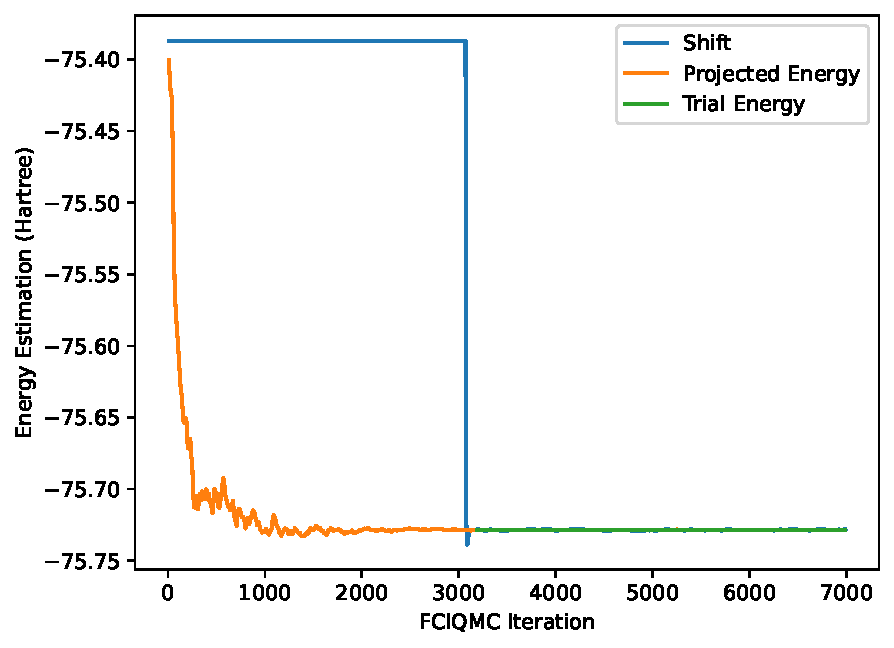
\includegraphics[width=0.9\textwidth]{figures/qmc/c2_example.pdf}
    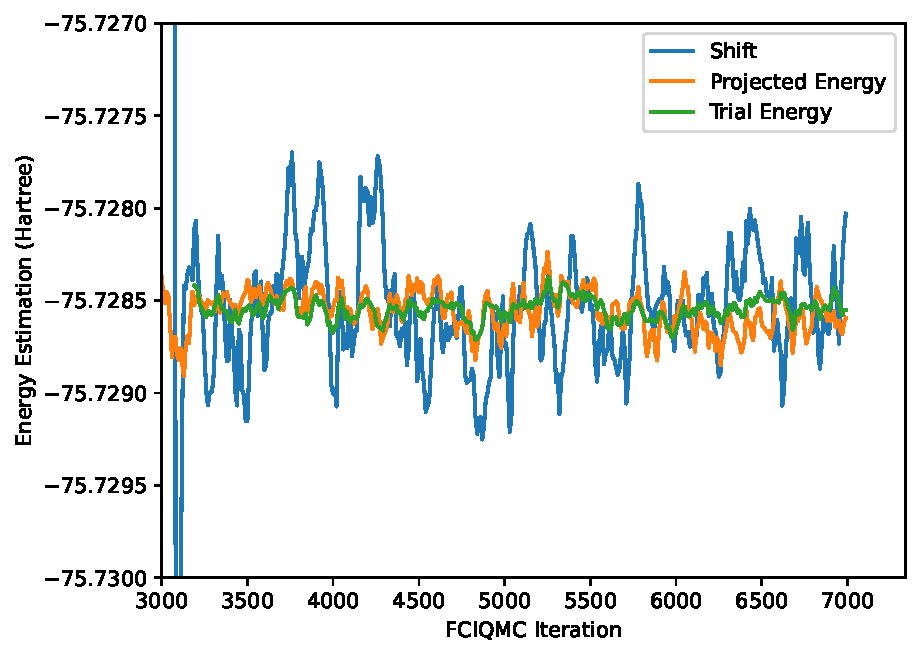
\includegraphics[width=0.9\textwidth]{figures/qmc/c2_example_zoomed.pdf}
    \caption{An example of the energy estimators used in an FCIQMC simulation. The shift is the most noisy, whereas the trial energy is the least noisy, but only available in variable shift mode and carries the highest cost. In this case, the trial energy is not a substantial improvement from the reference-projected energy. This calculation was done on the C$_2$ molecule with the \vdz basis, at equilibrium geometry, 1.2425 \AA.}
    \label{fig:fciqmc_energy_estimators}
\end{figure}

\subsection{Annihilation Plateaus}

\gls{FCIQMC} has its own kind of sign problem in the form of resolving the correct relative sign structure of the sampled states in the \gls{CI} vector.\supercite{spencerSignProblemPopulation2012} This manifests in the form of a so-called ``annihilation plateau'', illustrated in figure \ref{fig:annihilation_plateau}.

In this stage of the simulation, walkers are being spawned with incoherent signs, causing a massive amount of walker annihilation. This causes the population to stay relatively constant, until the sign structure is finally resolved and the population continues to grow again. The height of the plateau (i.e. the constant number of walkers where the simulation stagnates) quantifies the difficulty of the sign problem. In particular, for certain large systems, it can be prohibitively expensive to overcome. If we are below the annihilation plateau, then the original formulation of \gls{FCIQMC} is not reliable, as the correct sign structure is not yet resolved.

\begin{figure}[htbp]
    \centering
    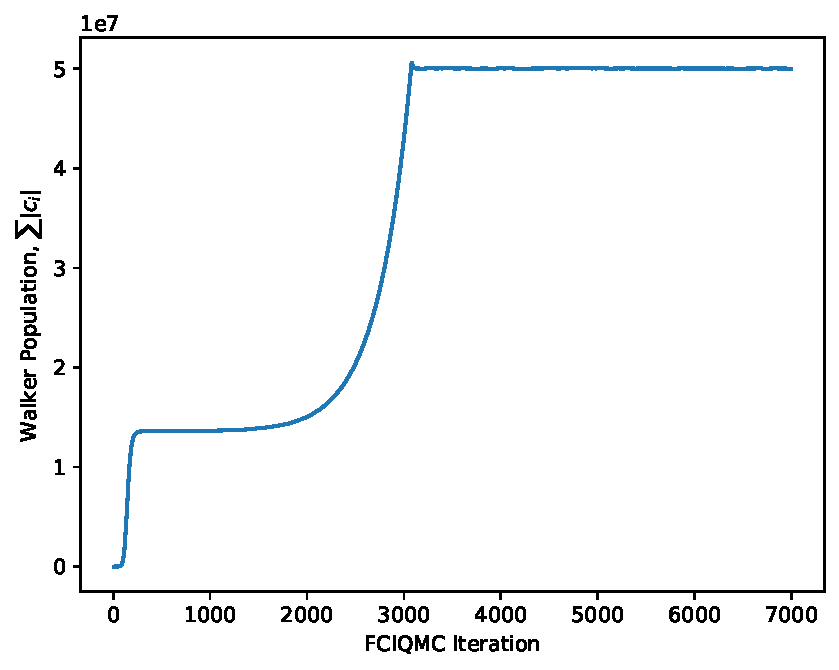
\includegraphics[width=0.9\textwidth]{figures/qmc/c2_example_plateau.pdf}
    \caption{An example of an annihilation plateau in the context of a \gls{FCIQMC} simulation. Despite not yet reaching the target population, the total population is roughly constant before increasing again. This stage is referred to as the annihilation plateau, and the higher the plateau, the more difficult the sign problem is. This calculation was done on the C$_2$ molecule with the \vdz basis, at equilibrium geometry, 1.2425 \AA. In this particular case, the plateau appears around $1.36\times 10^7$ walkers, and the target number is $5\times 10^7$.}
    \label{fig:annihilation_plateau}
\end{figure}

\subsection{The Initiator Approximation}

Since incoherent walker proliferation is a major source of the annihilation plateau, a sensible strategy to overcome this is by forcing growth to be coherent. This is achieved by the initiator approximation.\supercite{Cleland_initiator_2010} An \gls{FCIQMC} calculation with the initiator approximation is sometimes referred to as i-FCIQMC; however, since the approximation is so useful and ubiqituous, we simply referred to it as FCIQMC. Indeed, in this dissertation all FCIQMC calculations used the initiator approximation, unless otherwise specified.

The initiator approximation allows only those determinants (dubbed ``initiators'') with at least $N_\mathrm{thresh}$ walkers to spawn new walkers on unoccupied determinants. If the population is greater than this threshold, the assumption is that the (relative) sign of that state is correct, and hence the spawning event should produce the correct sign.

Since the approximation truncates spawning, the growth phase of the simulation is slower. However, the annihilation plateau disappears. Note that as $N_w\to\infty$, the initiator approximation becomes exact, as all sampled states are initiators. While there is a small bias introduced by the initiator approximation, the efficiency is greatly improved and the range of potential applications is greatly increased.

\subsection{Reduced Density Matrix Sampling}
\label{sec:fciqmc_rdm}
As described in section \ref{sec:density-matrices}, reduced density matrices are a useful tool for understanding the properties of a system. These can be sampled in \gls{FCIQMC} by considering the RDMs in the same basis.\supercite{overyUnbiased2014} The \gls{1RDM} is given by
\begin{equation}
    \gamma_{pq} = \sum_{ij} c_ic_j \bra{D_i}a_p^\dag a_q\ket{D_j}
\end{equation}
and the \gls{2RDM} by
\begin{equation}
    \Gamma_{pqrs} = \sum_{ijkl} c_ic_j \bra{D_i}a_p^\dag a_q^\dag a_s a_r\ket{D_j}.
\end{equation}
In FCIQMC, we have the \gls{CI} coefficients $c_i$ and $c_j$ by the walker distributions. However, using the same simulation for both $c_i$ and $c_j$ introduces a bias, hence to stochastically sample RDMs, we use an independent simultaneous simulation (referred to as a replica). One simulation samples $c_i$ whereas the other samples $c_j$. Since the statistical errors are independent, the overall error is reduced. Unfortunately this requires twice the computing power, but thankfully since the calculations are independent, they are trivially parallelisable.

Note also that by inserting the Hamiltonian (energy) operator into equation \ref{eq:rdm-expectation} and using the replica trick to obtain the RDMs, we can also obtain yet another energy measure in FCIQMC.

\subsection{Combining TC with Modern Electronic Structure}
\label{sec:tc-fciqmc}

The \gls{FCIQMC} algorithm may also be combined with the \gls{TC} method described in section \ref{sec:tc}.\supercite{Luo_tc_fciqmc_2018} Consider solving for the eigenstates $\Phi$ of the TC Hamiltonian $\htc$ using the imaginary-time Schr\"odinger equation,
\begin{equation}
    -\frac{\partial}{\partial\tau}\Phi = (\htc - S)\Phi.
\end{equation}
Since $\htc$ and $\hat H$ are isospectral, we have stationary states for the same values as the non-TC method. That is, we can control the walker population by setting the shift to the ground state energy, $S=E_0$.

The state $\Phi$ is described by a linear combination of \glspl{SD}, as in non-TC-FCIQMC,
\begin{equation}
    \ket\Phi = \sum_i c_i \ket{D_i}.
\end{equation}
However, since $\htc$ is non-Hermitian, the coefficients $\tilde c_i$ of the left-eigenvector with the same energy are not necessarily the same,
\begin{equation}
    \bra\Phi = \sum_i \tilde c_i \bra{D_i},
\end{equation}
and we must be careful when considering matrix connections $\bra{D_i}\htc\ket{D_j}$ and $\bra{D_j}\htc\ket{D_i}$. In particular, the probability of spawning a walker from $\ket{D_i}$ to $\ket{D_j}$ may not be the same as the probability of spawning from $\ket{D_j}$ to $\ket{D_i}$. Furthermore, when considering replicas such as in RDM sampling, the replica needs to be of the adjoint operator, $\htc^\dag$, in order to target $\tilde c_i$. This is accomplished by a simple transform of the Jastrow factor, $J\to -J$, though this may cause practical complications. Otherwise, \gls{FCIQMC} may be extended to \gls{TC} by simply applying the method directly to $\htc$. An appropriate transformation from $\hat H$ is therefore necessary beforehand.

Similar arguments may be made for applying \gls{TC} to \gls{CC} methods\supercite{schraivogelTranscorrelated2021,schraivogelTranscorrelated2023} and \gls{DMRG},\supercite{baiardiTranscorrelated2020} and \gls{TC} variants of these methods have already been developed and successfully applied. In addition to TC-FCIQMC, this also continues to be an active area of research.
